\documentclass{article}
\usepackage{graphicx} % Extended graphics inclusions
\usepackage{float}
\usepackage{url} % For \url{}
\usepackage{../config/atxy} % For front cover
\usepackage{amsfonts} % Needed for some fonts
\usepackage[usenames]{color} % Needed for colored R input/output
\usepackage{pdfcolmk} % Correct some problems with the color stack


\title{Importing sequences from flat files}

\author{Charif, D. \and Lobry, J.R.}

\usepackage{/Library/Frameworks/R.framework/Resources/share/texmf/Sweave}
\begin{document}
%
% To change the R input/output style:
%
\definecolor{Soutput}{rgb}{0,0,0.56}
\definecolor{Sinput}{rgb}{0.56,0,0}
\DefineVerbatimEnvironment{Sinput}{Verbatim}
{formatcom={\color{Sinput}},fontsize=\footnotesize, baselinestretch=0.75}
\DefineVerbatimEnvironment{Soutput}{Verbatim}
{formatcom={\color{Soutput}},fontsize=\footnotesize, baselinestretch=0.75}
%
% This removes the extra spacing after code and output chunks in Sweave,
% but keeps the spacing around the whole block.
%
\fvset{listparameters={\setlength{\topsep}{0pt}}}
\renewenvironment{Schunk}{\vspace{\topsep}}{\vspace{\topsep}}
%
% Rlogo
%
\newcommand{\Rlogo}{\protect
\includegraphics[height=1.8ex,keepaspectratio]{../figs/Rlogo.pdf}}
%
% Shortcut for seqinR:
%
\newcommand{\seqinr}{\texttt{seqin\bf{R}}}
\newcommand{\Seqinr}{\texttt{Seqin\bf{R}}}
\fvset{fontsize= \scriptsize}
%
% R output options and libraries to be loaded.
%
%
%  Sweave Options
%
% Put all figures in the fig folder and start the name with current file name.
% Do not produce EPS files
%


\maketitle
\tableofcontents
% BEGIN - DO NOT REMOVE THIS LINE


\section{Importing raw sequence data from FASTA files}

\subsection{FASTA files examples}

The FASTA format is very simple and widely used for simple import of
biological sequences. It was used originally by the FASTA program \cite{FASTA}.
It begins with a single-line description starting
with a character \texttt{'>'}, followed by lines of sequence data
of maximum 80 character each. Lines starting with a semi-colon
character \texttt{';'} are comment lines. Examples of files in FASTA format
are distributed with the \seqinr{} package in the \texttt{sequences}
directory:

\begin{Schunk}
\begin{Sinput}
 list.files(path = system.file("sequences", package = "seqinr"), 
     pattern = ".fasta")
\end{Sinput}
\begin{Soutput}
 [1] "ATH1_pep_cm_20040228.fasta" "Anouk.fasta"               
 [3] "bb.fasta"                   "bordetella.fasta"          
 [5] "ct.fasta"                   "ecolicgpe5.fasta"          
 [7] "gopher.fasta"               "humanMito.fasta"           
 [9] "legacy.fasta"               "louse.fasta"               
[11] "malM.fasta"                 "ortho.fasta"               
[13] "seqAA.fasta"                "smallAA.fasta"             
\end{Soutput}
\end{Schunk}

Here is an example of a FASTA file:

\begin{Schunk}
\begin{Sinput}
 cat(readLines(system.file("sequences/seqAA.fasta", package = "seqinr")), 
     sep = "\n")
\end{Sinput}
\begin{Soutput}
>A06852                  183 residues
MPRLFSYLLGVWLLLSQLPREIPGQSTNDFIKACGRELVRLWVEICGSVSWGRTALSLEE
PQLETGPPAETMPSSITKDAEILKMMLEFVPNLPQELKATLSERQPSLRELQQSASKDSN
LNFEEFKKIILNRQNEAEDKSLLELKNLGLDKHSRKKRLFRMTLSEKCCQVGCIRKDIAR
LC*
\end{Soutput}
\end{Schunk}

Here is an example of a FASTA file with comment lines:

\begin{Schunk}
\begin{Sinput}
 cat(readLines(system.file("sequences/legacy.fasta", package = "seqinr")), 
     sep = "\n")
\end{Sinput}
\begin{Soutput}
>LEGACY  921 bp
;
; Example of a FASTA file using comment lines starting with a semicolon
; as allowed in the original FASTA program:
;
;     if (line[0]!='>'&& line[0]!=';') {
;      for (i=l_offset; (n<maxs && rn < sstop)&&
;	     ((ic=qascii[line[i]&AAMASK])<EL); i++)
;	if (ic<NA && ++rn > sstart) seq[n++]= ic;
;      if (ic == ES || rn > sstop) break;
;    }
;
; From file getseq.c in FASTA program version 35.2.5
;
ATGAAAATGAATAAAAGTCTCATCGTCCTCTGTTTATCAGCAGGGTTACTGGCAAGCGCG
CCTGGAATTAGCCTTGCCGATGTTAACTACGTACCGCAAAACACCAGCGACGCGCCAGCC
ATTCCATCTGCTGCGCTGCAACAACTCACCTGGACACCGGTCGATCAATCTAAAACCCAG
ACCACCCAACTGGCGACCGGCGGCCAACAACTGAACGTTCCCGGCATCAGTGGTCCGGTT
GCTGCGTACAGCGTCCCGGCAAACATTGGCGAACTGACCCTGACGCTGACCAGCGAAGTG
AACAAACAAACCAGCGTTTTTGCGCCGAACGTGCTGATTCTTGATCAGAACATGACCCCA
TCAGCCTTCTTCCCCAGCAGTTATTTCACCTACCAGGAACCAGGCGTGATGAGTGCAGAT
CGGCTGGAAGGCGTTATGCGCCTGACACCGGCGTTGGGGCAGCAAAAACTTTATGTTCTG
GTCTTTACCACGGAAAAAGATCTCCAGCAGACGACCCAACTGCTCGACCCGGCTAAAGCC
TATGCCAAGGGCGTCGGTAACTCGATCCCGGATATCCCCGATCCGGTTGCTCGTCATACC
ACCGATGGCTTACTGAAACTGAAAGTGAAAACGAACTCCAGCTCCAGCGTGTTGGTAGGA
CCCTTATTTGGTTCCTCCGCTCCAGCTCCGGTTACGGTAGGTAACACGGCGGCACCAGCT
GTGGCTGCACCCGCTCCGGCACCGGTGAAGAAAAGCGAGCCGATGCTCAACGACACGGAA
AGTTATTTTAATACCGCGATCAAAAACGCTGTCGCGAAAGGTGATGTTGATAAGGCGTTA
AAACTGCTTGATGAAGCTGAACGCTTGGGATCGACATCTGCCCGTTCCACCTTTATCAGC
AGTGTAAAAGGCAAGGGGTAA
\end{Soutput}
\end{Schunk}

\subsection{The function \texttt{read.fasta()}}

The function \texttt{read.fasta()} imports sequences from FASTA files
into your workspace.

\subsubsection{DNA file example}

The example file looks like:

\begin{Schunk}
\begin{Sinput}
 dnafile <- system.file("sequences/malM.fasta", package = "seqinr")
 cat(readLines(dnafile), sep = "\n")
\end{Sinput}
\begin{Soutput}
>XYLEECOM.MALM  921 bp ACCESSION  E00218, X04477
ATGAAAATGAATAAAAGTCTCATCGTCCTCTGTTTATCAGCAGGGTTACTGGCAAGCGCG
CCTGGAATTAGCCTTGCCGATGTTAACTACGTACCGCAAAACACCAGCGACGCGCCAGCC
ATTCCATCTGCTGCGCTGCAACAACTCACCTGGACACCGGTCGATCAATCTAAAACCCAG
ACCACCCAACTGGCGACCGGCGGCCAACAACTGAACGTTCCCGGCATCAGTGGTCCGGTT
GCTGCGTACAGCGTCCCGGCAAACATTGGCGAACTGACCCTGACGCTGACCAGCGAAGTG
AACAAACAAACCAGCGTTTTTGCGCCGAACGTGCTGATTCTTGATCAGAACATGACCCCA
TCAGCCTTCTTCCCCAGCAGTTATTTCACCTACCAGGAACCAGGCGTGATGAGTGCAGAT
CGGCTGGAAGGCGTTATGCGCCTGACACCGGCGTTGGGGCAGCAAAAACTTTATGTTCTG
GTCTTTACCACGGAAAAAGATCTCCAGCAGACGACCCAACTGCTCGACCCGGCTAAAGCC
TATGCCAAGGGCGTCGGTAACTCGATCCCGGATATCCCCGATCCGGTTGCTCGTCATACC
ACCGATGGCTTACTGAAACTGAAAGTGAAAACGAACTCCAGCTCCAGCGTGTTGGTAGGA
CCCTTATTTGGTTCCTCCGCTCCAGCTCCGGTTACGGTAGGTAACACGGCGGCACCAGCT
GTGGCTGCACCCGCTCCGGCACCGGTGAAGAAAAGCGAGCCGATGCTCAACGACACGGAA
AGTTATTTTAATACCGCGATCAAAAACGCTGTCGCGAAAGGTGATGTTGATAAGGCGTTA
AAACTGCTTGATGAAGCTGAACGCTTGGGATCGACATCTGCCCGTTCCACCTTTATCAGC
AGTGTAAAAGGCAAGGGGTAA
\end{Soutput}
\end{Schunk}

With default arguments the output looks like:

\begin{Schunk}
\begin{Sinput}
 read.fasta(file = dnafile)
\end{Sinput}
\begin{Soutput}
$XYLEECOM.MALM
  [1] "a" "t" "g" "a" "a" "a" "a" "t" "g" "a" "a" "t" "a" "a" "a" "a" "g" "t"
 [19] "c" "t" "c" "a" "t" "c" "g" "t" "c" "c" "t" "c" "t" "g" "t" "t" "t" "a"
 [37] "t" "c" "a" "g" "c" "a" "g" "g" "g" "t" "t" "a" "c" "t" "g" "g" "c" "a"
 [55] "a" "g" "c" "g" "c" "g" "c" "c" "t" "g" "g" "a" "a" "t" "t" "a" "g" "c"
 [73] "c" "t" "t" "g" "c" "c" "g" "a" "t" "g" "t" "t" "a" "a" "c" "t" "a" "c"
 [91] "g" "t" "a" "c" "c" "g" "c" "a" "a" "a" "a" "c" "a" "c" "c" "a" "g" "c"
[109] "g" "a" "c" "g" "c" "g" "c" "c" "a" "g" "c" "c" "a" "t" "t" "c" "c" "a"
[127] "t" "c" "t" "g" "c" "t" "g" "c" "g" "c" "t" "g" "c" "a" "a" "c" "a" "a"
[145] "c" "t" "c" "a" "c" "c" "t" "g" "g" "a" "c" "a" "c" "c" "g" "g" "t" "c"
[163] "g" "a" "t" "c" "a" "a" "t" "c" "t" "a" "a" "a" "a" "c" "c" "c" "a" "g"
[181] "a" "c" "c" "a" "c" "c" "c" "a" "a" "c" "t" "g" "g" "c" "g" "a" "c" "c"
[199] "g" "g" "c" "g" "g" "c" "c" "a" "a" "c" "a" "a" "c" "t" "g" "a" "a" "c"
[217] "g" "t" "t" "c" "c" "c" "g" "g" "c" "a" "t" "c" "a" "g" "t" "g" "g" "t"
[235] "c" "c" "g" "g" "t" "t" "g" "c" "t" "g" "c" "g" "t" "a" "c" "a" "g" "c"
[253] "g" "t" "c" "c" "c" "g" "g" "c" "a" "a" "a" "c" "a" "t" "t" "g" "g" "c"
[271] "g" "a" "a" "c" "t" "g" "a" "c" "c" "c" "t" "g" "a" "c" "g" "c" "t" "g"
[289] "a" "c" "c" "a" "g" "c" "g" "a" "a" "g" "t" "g" "a" "a" "c" "a" "a" "a"
[307] "c" "a" "a" "a" "c" "c" "a" "g" "c" "g" "t" "t" "t" "t" "t" "g" "c" "g"
[325] "c" "c" "g" "a" "a" "c" "g" "t" "g" "c" "t" "g" "a" "t" "t" "c" "t" "t"
[343] "g" "a" "t" "c" "a" "g" "a" "a" "c" "a" "t" "g" "a" "c" "c" "c" "c" "a"
[361] "t" "c" "a" "g" "c" "c" "t" "t" "c" "t" "t" "c" "c" "c" "c" "a" "g" "c"
[379] "a" "g" "t" "t" "a" "t" "t" "t" "c" "a" "c" "c" "t" "a" "c" "c" "a" "g"
[397] "g" "a" "a" "c" "c" "a" "g" "g" "c" "g" "t" "g" "a" "t" "g" "a" "g" "t"
[415] "g" "c" "a" "g" "a" "t" "c" "g" "g" "c" "t" "g" "g" "a" "a" "g" "g" "c"
[433] "g" "t" "t" "a" "t" "g" "c" "g" "c" "c" "t" "g" "a" "c" "a" "c" "c" "g"
[451] "g" "c" "g" "t" "t" "g" "g" "g" "g" "c" "a" "g" "c" "a" "a" "a" "a" "a"
[469] "c" "t" "t" "t" "a" "t" "g" "t" "t" "c" "t" "g" "g" "t" "c" "t" "t" "t"
[487] "a" "c" "c" "a" "c" "g" "g" "a" "a" "a" "a" "a" "g" "a" "t" "c" "t" "c"
[505] "c" "a" "g" "c" "a" "g" "a" "c" "g" "a" "c" "c" "c" "a" "a" "c" "t" "g"
[523] "c" "t" "c" "g" "a" "c" "c" "c" "g" "g" "c" "t" "a" "a" "a" "g" "c" "c"
[541] "t" "a" "t" "g" "c" "c" "a" "a" "g" "g" "g" "c" "g" "t" "c" "g" "g" "t"
[559] "a" "a" "c" "t" "c" "g" "a" "t" "c" "c" "c" "g" "g" "a" "t" "a" "t" "c"
[577] "c" "c" "c" "g" "a" "t" "c" "c" "g" "g" "t" "t" "g" "c" "t" "c" "g" "t"
[595] "c" "a" "t" "a" "c" "c" "a" "c" "c" "g" "a" "t" "g" "g" "c" "t" "t" "a"
[613] "c" "t" "g" "a" "a" "a" "c" "t" "g" "a" "a" "a" "g" "t" "g" "a" "a" "a"
[631] "a" "c" "g" "a" "a" "c" "t" "c" "c" "a" "g" "c" "t" "c" "c" "a" "g" "c"
[649] "g" "t" "g" "t" "t" "g" "g" "t" "a" "g" "g" "a" "c" "c" "c" "t" "t" "a"
[667] "t" "t" "t" "g" "g" "t" "t" "c" "c" "t" "c" "c" "g" "c" "t" "c" "c" "a"
[685] "g" "c" "t" "c" "c" "g" "g" "t" "t" "a" "c" "g" "g" "t" "a" "g" "g" "t"
[703] "a" "a" "c" "a" "c" "g" "g" "c" "g" "g" "c" "a" "c" "c" "a" "g" "c" "t"
[721] "g" "t" "g" "g" "c" "t" "g" "c" "a" "c" "c" "c" "g" "c" "t" "c" "c" "g"
[739] "g" "c" "a" "c" "c" "g" "g" "t" "g" "a" "a" "g" "a" "a" "a" "a" "g" "c"
[757] "g" "a" "g" "c" "c" "g" "a" "t" "g" "c" "t" "c" "a" "a" "c" "g" "a" "c"
[775] "a" "c" "g" "g" "a" "a" "a" "g" "t" "t" "a" "t" "t" "t" "t" "a" "a" "t"
[793] "a" "c" "c" "g" "c" "g" "a" "t" "c" "a" "a" "a" "a" "a" "c" "g" "c" "t"
[811] "g" "t" "c" "g" "c" "g" "a" "a" "a" "g" "g" "t" "g" "a" "t" "g" "t" "t"
[829] "g" "a" "t" "a" "a" "g" "g" "c" "g" "t" "t" "a" "a" "a" "a" "c" "t" "g"
[847] "c" "t" "t" "g" "a" "t" "g" "a" "a" "g" "c" "t" "g" "a" "a" "c" "g" "c"
[865] "t" "t" "g" "g" "g" "a" "t" "c" "g" "a" "c" "a" "t" "c" "t" "g" "c" "c"
[883] "c" "g" "t" "t" "c" "c" "a" "c" "c" "t" "t" "t" "a" "t" "c" "a" "g" "c"
[901] "a" "g" "t" "g" "t" "a" "a" "a" "a" "g" "g" "c" "a" "a" "g" "g" "g" "g"
[919] "t" "a" "a"
attr(,"name")
[1] "XYLEECOM.MALM"
attr(,"Annot")
[1] ">XYLEECOM.MALM  921 bp ACCESSION  E00218, X04477"
attr(,"class")
[1] "SeqFastadna"
\end{Soutput}
\end{Schunk}

As from \seqinr{} 1.0-5 the automatic conversion of sequences into vector
of single characters can be neutralized, for instance:

\begin{Schunk}
\begin{Sinput}
 read.fasta(file = dnafile, as.string = TRUE)
\end{Sinput}
\begin{Soutput}
$XYLEECOM.MALM
[1] "atgaaaatgaataaaagtctcatcgtcctctgtttatcagcagggttactggcaagcgcgcctggaattagccttgccgatgttaactacgtaccgcaaaacaccagcgacgcgccagccattccatctgctgcgctgcaacaactcacctggacaccggtcgatcaatctaaaacccagaccacccaactggcgaccggcggccaacaactgaacgttcccggcatcagtggtccggttgctgcgtacagcgtcccggcaaacattggcgaactgaccctgacgctgaccagcgaagtgaacaaacaaaccagcgtttttgcgccgaacgtgctgattcttgatcagaacatgaccccatcagccttcttccccagcagttatttcacctaccaggaaccaggcgtgatgagtgcagatcggctggaaggcgttatgcgcctgacaccggcgttggggcagcaaaaactttatgttctggtctttaccacggaaaaagatctccagcagacgacccaactgctcgacccggctaaagcctatgccaagggcgtcggtaactcgatcccggatatccccgatccggttgctcgtcataccaccgatggcttactgaaactgaaagtgaaaacgaactccagctccagcgtgttggtaggacccttatttggttcctccgctccagctccggttacggtaggtaacacggcggcaccagctgtggctgcacccgctccggcaccggtgaagaaaagcgagccgatgctcaacgacacggaaagttattttaataccgcgatcaaaaacgctgtcgcgaaaggtgatgttgataaggcgttaaaactgcttgatgaagctgaacgcttgggatcgacatctgcccgttccacctttatcagcagtgtaaaaggcaaggggtaa"
attr(,"name")
[1] "XYLEECOM.MALM"
attr(,"Annot")
[1] ">XYLEECOM.MALM  921 bp ACCESSION  E00218, X04477"
attr(,"class")
[1] "SeqFastadna"
\end{Soutput}
\end{Schunk}

Forcing to lower case letters can be disabled this way:

\begin{Schunk}
\begin{Sinput}
 read.fasta(file = dnafile, as.string = TRUE, forceDNAtolower = FALSE)
\end{Sinput}
\begin{Soutput}
$XYLEECOM.MALM
[1] "ATGAAAATGAATAAAAGTCTCATCGTCCTCTGTTTATCAGCAGGGTTACTGGCAAGCGCGCCTGGAATTAGCCTTGCCGATGTTAACTACGTACCGCAAAACACCAGCGACGCGCCAGCCATTCCATCTGCTGCGCTGCAACAACTCACCTGGACACCGGTCGATCAATCTAAAACCCAGACCACCCAACTGGCGACCGGCGGCCAACAACTGAACGTTCCCGGCATCAGTGGTCCGGTTGCTGCGTACAGCGTCCCGGCAAACATTGGCGAACTGACCCTGACGCTGACCAGCGAAGTGAACAAACAAACCAGCGTTTTTGCGCCGAACGTGCTGATTCTTGATCAGAACATGACCCCATCAGCCTTCTTCCCCAGCAGTTATTTCACCTACCAGGAACCAGGCGTGATGAGTGCAGATCGGCTGGAAGGCGTTATGCGCCTGACACCGGCGTTGGGGCAGCAAAAACTTTATGTTCTGGTCTTTACCACGGAAAAAGATCTCCAGCAGACGACCCAACTGCTCGACCCGGCTAAAGCCTATGCCAAGGGCGTCGGTAACTCGATCCCGGATATCCCCGATCCGGTTGCTCGTCATACCACCGATGGCTTACTGAAACTGAAAGTGAAAACGAACTCCAGCTCCAGCGTGTTGGTAGGACCCTTATTTGGTTCCTCCGCTCCAGCTCCGGTTACGGTAGGTAACACGGCGGCACCAGCTGTGGCTGCACCCGCTCCGGCACCGGTGAAGAAAAGCGAGCCGATGCTCAACGACACGGAAAGTTATTTTAATACCGCGATCAAAAACGCTGTCGCGAAAGGTGATGTTGATAAGGCGTTAAAACTGCTTGATGAAGCTGAACGCTTGGGATCGACATCTGCCCGTTCCACCTTTATCAGCAGTGTAAAAGGCAAGGGGTAA"
attr(,"name")
[1] "XYLEECOM.MALM"
attr(,"Annot")
[1] ">XYLEECOM.MALM  921 bp ACCESSION  E00218, X04477"
attr(,"class")
[1] "SeqFastadna"
\end{Soutput}
\end{Schunk}


\subsubsection{Protein file example}

The example file looks like:

\begin{Schunk}
\begin{Sinput}
 aafile <- system.file("sequences/seqAA.fasta", package = "seqinr")
 cat(readLines(aafile), sep = "\n")
\end{Sinput}
\begin{Soutput}
>A06852                  183 residues
MPRLFSYLLGVWLLLSQLPREIPGQSTNDFIKACGRELVRLWVEICGSVSWGRTALSLEE
PQLETGPPAETMPSSITKDAEILKMMLEFVPNLPQELKATLSERQPSLRELQQSASKDSN
LNFEEFKKIILNRQNEAEDKSLLELKNLGLDKHSRKKRLFRMTLSEKCCQVGCIRKDIAR
LC*
\end{Soutput}
\end{Schunk}

Read the protein sequence file, looks like:

\begin{Schunk}
\begin{Sinput}
 read.fasta(aafile, seqtype = "AA")
\end{Sinput}
\begin{Soutput}
$A06852
  [1] "M" "P" "R" "L" "F" "S" "Y" "L" "L" "G" "V" "W" "L" "L" "L" "S" "Q" "L"
 [19] "P" "R" "E" "I" "P" "G" "Q" "S" "T" "N" "D" "F" "I" "K" "A" "C" "G" "R"
 [37] "E" "L" "V" "R" "L" "W" "V" "E" "I" "C" "G" "S" "V" "S" "W" "G" "R" "T"
 [55] "A" "L" "S" "L" "E" "E" "P" "Q" "L" "E" "T" "G" "P" "P" "A" "E" "T" "M"
 [73] "P" "S" "S" "I" "T" "K" "D" "A" "E" "I" "L" "K" "M" "M" "L" "E" "F" "V"
 [91] "P" "N" "L" "P" "Q" "E" "L" "K" "A" "T" "L" "S" "E" "R" "Q" "P" "S" "L"
[109] "R" "E" "L" "Q" "Q" "S" "A" "S" "K" "D" "S" "N" "L" "N" "F" "E" "E" "F"
[127] "K" "K" "I" "I" "L" "N" "R" "Q" "N" "E" "A" "E" "D" "K" "S" "L" "L" "E"
[145] "L" "K" "N" "L" "G" "L" "D" "K" "H" "S" "R" "K" "K" "R" "L" "F" "R" "M"
[163] "T" "L" "S" "E" "K" "C" "C" "Q" "V" "G" "C" "I" "R" "K" "D" "I" "A" "R"
[181] "L" "C" "*"
attr(,"name")
[1] "A06852"
attr(,"Annot")
[1] ">A06852                  183 residues"
attr(,"class")
[1] "SeqFastaAA"
\end{Soutput}
\end{Schunk}

The same, but as string and without attributes setting, looks like:

\begin{Schunk}
\begin{Sinput}
 read.fasta(aafile, seqtype = "AA", as.string = TRUE, set.attributes = FALSE)
\end{Sinput}
\begin{Soutput}
$A06852
[1] "MPRLFSYLLGVWLLLSQLPREIPGQSTNDFIKACGRELVRLWVEICGSVSWGRTALSLEEPQLETGPPAETMPSSITKDAEILKMMLEFVPNLPQELKATLSERQPSLRELQQSASKDSNLNFEEFKKIILNRQNEAEDKSLLELKNLGLDKHSRKKRLFRMTLSEKCCQVGCIRKDIARLC*"
\end{Soutput}
\end{Schunk}

\subsection{The function \texttt{write.fasta()}}

This function writes sequences to a file in FASTA format.
Read 3 coding sequences sequences from a FASTA file:

\begin{Schunk}
\begin{Sinput}
 ortho <- read.fasta(file = system.file("sequences/ortho.fasta", 
     package = "seqinr"))
 length(ortho)
\end{Sinput}
\begin{Soutput}
[1] 3
\end{Soutput}
\begin{Sinput}
 ortho[[1]][1:12]
\end{Sinput}
\begin{Soutput}
 [1] "a" "t" "g" "g" "c" "t" "c" "a" "g" "c" "g" "g"
\end{Soutput}
\end{Schunk}

Select only third codon positions:

\begin{Schunk}
\begin{Sinput}
 ortho3 <- lapply(ortho, function(x) x[seq(from = 3, to = length(x), 
     by = 3)])
 ortho3[[1]][1:4]
\end{Sinput}
\begin{Soutput}
[1] "g" "t" "g" "g"
\end{Soutput}
\end{Schunk}

Write the modified sequences to a file:

\begin{Schunk}
\begin{Sinput}
 tmpf <- tempfile()
 write.fasta(sequences = ortho3, names = names(ortho3), nbchar = 80, 
     file.out = tmpf)
\end{Sinput}
\end{Schunk}

Read them again from the same file and check that sequences are preserved:

\begin{Schunk}
\begin{Sinput}
 ortho3bis <- read.fasta(tmpf, set.attributes = FALSE)
 identical(ortho3bis, ortho3)
\end{Sinput}
\begin{Soutput}
[1] TRUE
\end{Soutput}
\end{Schunk}

\subsection{Big room examples}

\subsubsection{Oriloc example (\textit{Chlamydia trachomatis} complete genome)}

A more consequent example is given in the fasta file \texttt{ct.fasta} which
contains the complete genome of \textit{Chlamydia trachomatis} that was
used in \cite{oriloc}. You should be able to reproduce figure 1b from this
paper with the following code:

\begin{Schunk}
\begin{Sinput}
 out <- oriloc(seq.fasta = system.file("sequences/ct.fasta", 
     package = "seqinr"), g2.coord = system.file("sequences/ct.coord", 
     package = "seqinr"), oldoriloc = TRUE)
 plot(out$st, out$sk/1000, type = "l", xlab = "Map position in Kb", 
     ylab = "Cumulated composite skew in Kb", main = expression(italic(Chlamydia ~ 
         ~trachomatis) ~ ~complete ~ ~genome), las = 1)
 abline(h = 0, lty = 2)
 text(400, -4, "Terminus")
 text(850, 9, "Origin")
\end{Sinput}
\end{Schunk}
\includegraphics{../figs/getseqflat-oriloc}

Note that the algorithm has been improved since then and that it's
more advisable to use the default option \texttt{oldoriloc = FALSE}
if you are interested in the prediction of origins and terminus of
replication from base composition biases (more on this at
\url{http://pbil.univ-lyon1.fr/software/oriloc.html}). See also \cite{smorfland}
for a recent review on this topic.

\begin{Schunk}
\begin{Sinput}
 out <- oriloc(seq.fasta = system.file("sequences/ct.fasta", 
     package = "seqinr"), g2.coord = system.file("sequences/ct.coord", 
     package = "seqinr"))
 plot(out$st, out$sk/1000, type = "l", xlab = "Map position in Kb", 
     ylab = "Cumulated composite skew in Kb", main = expression(italic(Chlamydia ~ 
         ~trachomatis) ~ ~complete ~ ~genome), las = 1)
 mtext("New version")
 abline(h = 0, lty = 2)
 text(400, -4, "Terminus")
 text(850, 9, "Origin")
\end{Sinput}
\end{Schunk}
\includegraphics{../figs/getseqflat-oriloc2}

\subsubsection{Example with 21,161 proteins from \textit{Arabidobpsis thaliana}}

As from \seqinr{} 1.0-5 the automatic conversion of sequences into vector
of single characters and the automatic attribute settings can be neutralized, for
instance :

\begin{Schunk}
\begin{Sinput}
 smallAA <- system.file("sequences/smallAA.fasta", package = "seqinr")
 read.fasta(smallAA, seqtype = "AA", as.string = TRUE, set.attributes = FALSE)
\end{Sinput}
\begin{Soutput}
$smallAA
[1] "SEQINRSEQINRSEQINRSEQINR*"
\end{Soutput}
\end{Schunk}

This is interesting to save time and space when reading large FASTA files.
\marginpar{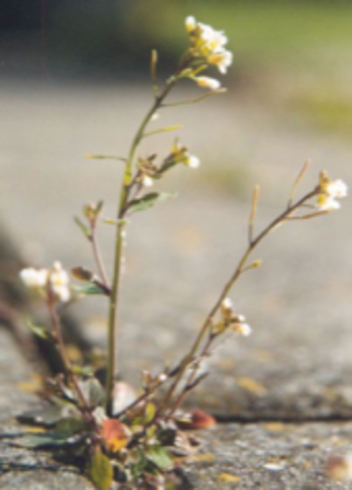
\includegraphics[width=\marginparwidth]{../figs/ath}\\
\tiny{\textit{Arabidobpsis thaliana}. Source: wikipedia.}
}
Let's give a practical example. In their paper \cite{HannahMA2005},
Matthew Hannah, Arnd Heyer and Dirk Hincha were working on
\textit{Arabidobpsis thaliana} genes in order to detect those involved
in cold acclimation. They were interested by the detection of proteins called
hydrophilins, that had a mean hydrophilicity of over 1 and glycine
content of over 0.08 \cite{GarayArroyoA2000}, because they are though to be important
for freezing tolerance. The starting point was a FASTA file called
\texttt{ATH1\_pep\_cm\_20040228} downloaded from the Arabidopsis
Information Ressource (TAIR at \url{http://www.arabidopsis.org/}) 
which contains the sequences of 21,161 proteins.

\begin{Schunk}
\begin{Sinput}
 athfile <- system.file("sequences/ATH1_pep_cm_20040228.fasta", 
     package = "seqinr")
 system.time(ath <- read.fasta(athfile, seqtype = "AA", as.string = TRUE, 
     set.attributes = FALSE))
\end{Sinput}
\begin{Soutput}
   user  system elapsed 
  5.781   0.134   6.407 
\end{Soutput}
\end{Schunk}

It's about 10 seconds here to read 21,161 protein sequences. We save them
in XDR binary format\footnote{
this is a multi-platform compatible binary format: you can save data
under unix and load them under Mac OS X, for instance, without problem.
} to read them faster later at will:

\begin{Schunk}
\begin{Sinput}
 save(ath, file = "ath.RData")
\end{Sinput}
\end{Schunk}
\begin{Schunk}
\begin{Sinput}
 system.time(load("ath.RData"))
\end{Sinput}
\begin{Soutput}
   user  system elapsed 
  0.329   0.009   0.341 
\end{Soutput}
\end{Schunk}

Now it's less than a second to load the whole data set thanks to the XDR format.
The object size is about 15 Mo in RAM, that is something very close to
the flat file size on disk:

\begin{Schunk}
\begin{Sinput}
 object.size(ath)/2^20
\end{Sinput}
\begin{Soutput}
[1] 14.65537
\end{Soutput}
\begin{Sinput}
 file.info(athfile)$size/2^20
\end{Sinput}
\begin{Soutput}
[1] 15.89863
\end{Soutput}
\end{Schunk}

Using strings for sequence storage is very comfortable when there is
an efficient function to compute what you want. For instance, suppose
that you are interested by the distribution of protein size in
\textit{Arabidopsis thaliana}. There is an efficient vectorized function
called \texttt{nchar()} that will do the job, we just have to remove
one unit because of the stop codon which is translated as a star (*) in
this data set. This is a simple and direct task under \Rlogo{}:

\begin{Schunk}
\begin{Sinput}
 nres <- nchar(ath) - 1
 hist(log10(nres), col = grey(0.7), xlab = "Protein size (log10 scale)", 
     ylab = "Protein count", main = expression(italic(Arabidopsis ~ 
         ~thaliana)))
\end{Sinput}
\end{Schunk}
\includegraphics{../figs/getseqflat-athdistriprotsize}

However, sometimes it is more convenient to work with the single
character vector representation of sequences. For instance, to count
the number of glycine (G), we first play with one sequence, let's
take the smallest one in the data set:

\begin{Schunk}
\begin{Sinput}
 which.min(nres)
\end{Sinput}
\begin{Soutput}
At2g25990.1 
       9523 
\end{Soutput}
\begin{Sinput}
 ath[[9523]]
\end{Sinput}
\begin{Soutput}
[1] "MAGSQREKLKPRTKGSTRC*"
\end{Soutput}
\begin{Sinput}
 s2c(ath[[9523]])
\end{Sinput}
\begin{Soutput}
 [1] "M" "A" "G" "S" "Q" "R" "E" "K" "L" "K" "P" "R" "T" "K" "G" "S" "T" "R"
[19] "C" "*"
\end{Soutput}
\begin{Sinput}
 s2c(ath[[9523]]) == "G"
\end{Sinput}
\begin{Soutput}
 [1] FALSE FALSE  TRUE FALSE FALSE FALSE FALSE FALSE FALSE FALSE FALSE FALSE
[13] FALSE FALSE  TRUE FALSE FALSE FALSE FALSE FALSE
\end{Soutput}
\begin{Sinput}
 sum(s2c(ath[[9523]]) == "G")
\end{Sinput}
\begin{Soutput}
[1] 2
\end{Soutput}
\end{Schunk}

We can now easily define a vectorised function to count the number
of glycine:

\begin{Schunk}
\begin{Sinput}
 ngly <- function(data) {
     res <- sapply(data, function(x) sum(s2c(x) == "G"))
     names(res) <- NULL
     return(res)
 }
\end{Sinput}
\end{Schunk}

Now we can use \texttt{ngly()} in the same way that \texttt{nchar()} so
that computing glycine frequencies is very simple:

\begin{Schunk}
\begin{Sinput}
 ngly(ath[1:10])
\end{Sinput}
\begin{Soutput}
 [1]  25   5  29 128   8  27  27  26  21  18
\end{Soutput}
\begin{Sinput}
 fgly <- ngly(ath)/nres
\end{Sinput}
\end{Schunk}

And we can have a look at the distribution:

\begin{Schunk}
\begin{Sinput}
 hist(fgly, col = grey(0.7), main = "Distribution of Glycine frequency", 
     xlab = "Glycine content", ylab = "Protein count")
 abline(v = 0.08, col = "red")
 legend("topright", inset = 0.01, lty = 1, col = "red", legend = "Threshold for hydrophilines")
\end{Sinput}
\end{Schunk}
\includegraphics{../figs/getseqflat-histgly}

Let's use a boxplot instead:

\begin{Schunk}
\begin{Sinput}
 boxplot(fgly, horizontal = TRUE, col = grey(0.7), main = "Distribution of Glycine frequency", 
     xlab = "Glycine content", ylab = "Protein count")
 abline(v = 0.08, col = "red")
 legend("topright", inset = 0.01, lty = 1, col = "red", legend = "Threshold for hydrophilines")
\end{Sinput}
\end{Schunk}
\includegraphics{../figs/getseqflat-boxplotgly}

The threshold value for the glycine content in hydrophilines is therefore
very close to the third quartile of the distribution:

\begin{Schunk}
\begin{Sinput}
 summary(fgly)
\end{Sinput}
\begin{Soutput}
   Min. 1st Qu.  Median    Mean 3rd Qu.    Max. 
0.00000 0.04907 0.06195 0.06475 0.07639 0.59240 
\end{Soutput}
\end{Schunk}

We want now to compute something relatively more complex,
we want the Kyte and Doolittle \cite{KD} hydropathy score of our proteins
(aka GRAVY score). This is basically a linear form on amino
acid frequencies:

$$
s = \sum_{i = 1}^{20} \alpha_{i}f_{i}
$$
where $\alpha_{i}$ is the coefficient for amino acid number $i$ and
$f_{i}$ the relative frequency of amino acid number $i$. The coefficients
$\alpha_{i}$ are given in the \texttt{KD} component of the data set
\texttt{EXP}:

\begin{Schunk}
\begin{Sinput}
 data(EXP)
 EXP$KD
\end{Sinput}
\begin{Soutput}
 [1] -3.9 -3.5 -3.9 -3.5 -0.7 -0.7 -0.7 -0.7 -4.5 -0.8 -4.5 -0.8  4.5  4.5
[15]  1.9  4.5 -3.5 -3.2 -3.5 -3.2 -1.6 -1.6 -1.6 -1.6 -4.5 -4.5 -4.5 -4.5
[29]  3.8  3.8  3.8  3.8 -3.5 -3.5 -3.5 -3.5  1.8  1.8  1.8  1.8 -0.4 -0.4
[43] -0.4 -0.4  4.2  4.2  4.2  4.2  0.0 -1.3  0.0 -1.3 -0.8 -0.8 -0.8 -0.8
[57]  0.0  2.5 -0.9  2.5  3.8  2.8  3.8  2.8
\end{Soutput}
\end{Schunk}

This is for codons in lexical order, that is:

\begin{Schunk}
\begin{Sinput}
 words()
\end{Sinput}
\begin{Soutput}
 [1] "aaa" "aac" "aag" "aat" "aca" "acc" "acg" "act" "aga" "agc" "agg" "agt"
[13] "ata" "atc" "atg" "att" "caa" "cac" "cag" "cat" "cca" "ccc" "ccg" "cct"
[25] "cga" "cgc" "cgg" "cgt" "cta" "ctc" "ctg" "ctt" "gaa" "gac" "gag" "gat"
[37] "gca" "gcc" "gcg" "gct" "gga" "ggc" "ggg" "ggt" "gta" "gtc" "gtg" "gtt"
[49] "taa" "tac" "tag" "tat" "tca" "tcc" "tcg" "tct" "tga" "tgc" "tgg" "tgt"
[61] "tta" "ttc" "ttg" "ttt"
\end{Soutput}
\end{Schunk}

But since we are working with protein sequences here we name the
coefficient according to their amino acid :

\begin{Schunk}
\begin{Sinput}
 names(EXP$KD) <- sapply(words(), function(x) translate(s2c(x)))
\end{Sinput}
\end{Schunk}

We just need one value per amino acid, we sort them in the lexical
order, and we reverse the scale so as to have positive values for
hydrophilic proteins as in \cite{HannahMA2005} :

\begin{Schunk}
\begin{Sinput}
 kdc <- EXP$KD[unique(names(EXP$KD))]
 kdc <- -kdc[order(names(kdc))]
 kdc
\end{Sinput}
\begin{Soutput}
   *    A    C    D    E    F    G    H    I    K    L    M    N    P    Q 
 0.0 -1.8 -2.5  3.5  3.5 -2.8  0.4  3.2 -4.5  3.9 -3.8 -1.9  3.5  1.6  3.5 
   R    S    T    V    W    Y 
 4.5  0.8  0.7 -4.2  0.9  1.3 
\end{Soutput}
\end{Schunk}

Now that we have the vector of coefficient $\alpha_{i}$, we need the
amino acid relative frequencies $f_{i}$, let's play with one protein
first:

\begin{Schunk}
\begin{Sinput}
 ath[[9523]]
\end{Sinput}
\begin{Soutput}
[1] "MAGSQREKLKPRTKGSTRC*"
\end{Soutput}
\begin{Sinput}
 s2c(ath[[9523]])
\end{Sinput}
\begin{Soutput}
 [1] "M" "A" "G" "S" "Q" "R" "E" "K" "L" "K" "P" "R" "T" "K" "G" "S" "T" "R"
[19] "C" "*"
\end{Soutput}
\begin{Sinput}
 table(s2c(ath[[9523]]))
\end{Sinput}
\begin{Soutput}
* A C E G K L M P Q R S T 
1 1 1 1 2 3 1 1 1 1 3 2 2 
\end{Soutput}
\begin{Sinput}
 table(factor(s2c(ath[[9523]]), levels = names(kdc)))
\end{Sinput}
\begin{Soutput}
* A C D E F G H I K L M N P Q R S T V W Y 
1 1 1 0 1 0 2 0 0 3 1 1 0 1 1 3 2 2 0 0 0 
\end{Soutput}
\end{Schunk}

Now that we know how to count amino acids it's relatively easy thanks
to R's matrix operator \texttt{\%*\%} to
define a vectorised function to compute a linear form on amino acid
frequencies:

\begin{Schunk}
\begin{Sinput}
 linform <- function(data, coef) {
     f <- function(x) {
         aaseq <- s2c(x)
         freq <- table(factor(aaseq, levels = names(coef)))/length(aaseq)
         return(coef %*% freq)
     }
     res <- sapply(data, f)
     names(res) <- NULL
     return(res)
 }
 kdath <- linform(ath, kdc)
\end{Sinput}
\end{Schunk}

Let's have a look at the distribution:

\begin{Schunk}
\begin{Sinput}
 boxplot(kdath, horizontal = TRUE, col = grey(0.7), main = "Distribution of Hydropathy index", 
     xlab = "Kyte and Doolittle GRAVY score")
 abline(v = 1, col = "red")
 legend("topleft", inset = 0.01, lty = 1, col = "red", legend = "Threshold for hydrophilines")
\end{Sinput}
\end{Schunk}
\includegraphics{../figs/getseqflat-distriKD}

The threshold is therefore much more stringent here than the previous one on
glycine content. Let's define a vector of logicals to select the hydrophilines:

\begin{Schunk}
\begin{Sinput}
 hydrophilines <- fgly > 0.08 & kdath > 1
 head(names(ath)[hydrophilines])
\end{Sinput}
\begin{Soutput}
[1] "At1g02840.1" "At1g02840.2" "At1g02840.3" "At1g03320.1" "At1g03820.1"
[6] "At1g04450.1"
\end{Soutput}
\end{Schunk}

Check with a simple graph that there is no mistake here:

\begin{Schunk}
\begin{Sinput}
 library(MASS)
 dst <- kde2d(kdath, fgly, n = 50)
 filled.contour(x = dst, color.palette = topo.colors, plot.axes = {
     axis(1)
     axis(2)
     title(xlab = "Kyte and Doolittle GRAVY score", ylab = "Glycine content", 
         main = "Hydrophilines location")
     abline(v = 1, col = "yellow")
     abline(h = 0.08, col = "yellow")
     points(kdath[hydrophilines], fgly[hydrophilines], col = "white")
     legend("topleft", inset = 0.02, lty = 1, col = "yellow", 
         bg = "white", legend = "Threshold for hydrophilines", 
         cex = 0.8)
 })
\end{Sinput}
\end{Schunk}
\includegraphics{../figs/getseqflat-chekhydro}

Everything seems to be OK, we can save the results in a data frame:

\begin{Schunk}
\begin{Sinput}
 athres <- data.frame(list(name = names(ath), KD = kdath, Gly = fgly))
 head(athres)
\end{Sinput}
\begin{Soutput}
                   name         KD        Gly
At1g01010.1 At1g01010.1  0.7297674 0.05827506
At1g01020.1 At1g01020.1 -0.1674419 0.03906250
At1g01030.1 At1g01030.1  0.8136490 0.08100559
At1g01040.1 At1g01040.1  0.4159686 0.06705081
At1g01050.1 At1g01050.1  0.4460094 0.03773585
At1g01060.1 At1g01060.1  0.7444272 0.04186047
\end{Soutput}
\end{Schunk}

  
%
% Deleted because this table is a little bit too long
%
% We can also export the data frame in a \LaTeX~table:
%
%<<hydlatex,fig=F,eval=T>>=
%library(xtable)
%print(xtable(x = hyd, caption = "Hydrophilines from \\textit{Arabidopsis thaliana}.", 
%    label = "hyd", digits = c(0,0,0,3,3)), file = "hyd.tex", size = "tiny")
%@
%\input{hyd.tex}
%
%so as to generate table \ref{hyd}.

We want to check now that the results are consistent with those reported
previously. The following table is extracted from the file
\texttt{pgen.0010026.st003.xls} provided as the supplementary
material table S3 in \cite{HannahMA2005} and available at
\url{http://www.pubmedcentral.nih.gov/picrender.fcgi?artid=1189076&blobname=pgen.0010026.st003.xls}.
Only the protein names, the hydrophilicity and the glycine content were
extracted:

\begin{Schunk}
\begin{Sinput}
 hannah <- read.table(system.file("sequences/hannah.txt", package = "seqinr"), 
     sep = "\t", header = TRUE)
 head(hannah)
\end{Sinput}
\begin{Soutput}
        AGI Hydrophilicity Glycine
1 At2g19570          -0.10    0.07
2 At2g45290          -0.25    0.09
3 At4g29570          -0.05    0.07
4 At4g29580          -0.10    0.06
5 At4g29600          -0.14    0.06
6 At5g28050          -0.11    0.08
\end{Soutput}
\end{Schunk}

The protein names are not exactly the same because they have no extension.
As explained in \cite{HannahMA2005}, when multiple gene models 
were predicted only the first was one used. Then:

\begin{Schunk}
\begin{Sinput}
 hannah$AGI <- paste(hannah$AGI, "1", sep = ".")
 head(hannah)
\end{Sinput}
\begin{Soutput}
          AGI Hydrophilicity Glycine
1 At2g19570.1          -0.10    0.07
2 At2g45290.1          -0.25    0.09
3 At4g29570.1          -0.05    0.07
4 At4g29580.1          -0.10    0.06
5 At4g29600.1          -0.14    0.06
6 At5g28050.1          -0.11    0.08
\end{Soutput}
\end{Schunk}

We join now the two data frames thanks to their common key:

\begin{Schunk}
\begin{Sinput}
 join <- merge(hannah, athres, by.x = "AGI", by.y = "name")
 head(join)
\end{Sinput}
\begin{Soutput}
          AGI Hydrophilicity Glycine         KD        Gly
1 At1g01120.1          -0.10    0.06 0.10699433 0.05871212
2 At1g01390.1           0.02    0.06 0.00914761 0.06458333
3 At1g01390.1           0.02    0.06 0.00914761 0.06458333
4 At1g01420.1          -0.05    0.07 0.06203320 0.07276507
5 At1g01420.1          -0.05    0.07 0.06203320 0.07276507
6 At1g01480.1          -0.20    0.07 0.20080483 0.06653226
\end{Soutput}
\end{Schunk}

Let's compare the glycine content :

\begin{Schunk}
\begin{Sinput}
 plot(join$Glycine, join$Gly, xlab = "Glycine content in Hannah et al. (2005)", 
     ylab = "Glycine content here", main = "Comparison of Glycine content results")
 abline(c(0, 1), col = "red")
\end{Sinput}
\end{Schunk}
\includegraphics{../figs/getseqflat-comparegly}

The results are consistent, we have just lost some resolution because
there are only two figures after the decimal point in the Excel\footnote{
this software is a real \textbf{pain} for the reproducibility of results.
This is well documented, see \url{http://www.burns-stat.com/pages/Tutor/spreadsheet_addiction.html}
and references therein.
} file. Let's have a look at the GRAVY score now:

\begin{Schunk}
\begin{Sinput}
 plot(join$Hydrophilicity, join$KD, xlab = "GRAVY score in Hannah et al. (2005)", 
     ylab = "GRAVY score here", main = "Comparison of hydropathy score results", 
     las = 1)
 abline(c(0, -1), col = "red")
 abline(v = 0, lty = 2)
 abline(h = 0, lty = 2)
\end{Sinput}
\end{Schunk}
\includegraphics{../figs/getseqflat-comparekd}

The results are consistent, it's hard to say whether the small differences
are due to Excel rounding errors or because the method used to compute the GRAVY
score was not exactly the same (in \cite{HannahMA2005} they used the
mean over a sliding window). 


\section{Importing aligned sequence data}

\subsection{Aligned sequences files examples}

\subsubsection{mase}

Mase format is a flatfile format use by the SeaView multiple alignment 
editor \cite{SeaView}, developed by Manolo Gouy and available at
\url{http://pbil.univ-lyon1.fr/software/seaview.html}.
The mase format is used to store nucleotide or protein multiple alignments. 
The beginning of the file must contain a header containing at least one line 
(but the content of this header may be empty). The header lines must 
begin by ;;. The body of the file has the following structure: First, each 
entry must begin by one (or more) commentary line. Commentary lines 
begin by the character ;. Again, this commentary line may be empty. 
After the commentaries, the name of the sequence is written on a separate line. 
At last, the sequence itself is written on the following lines.

\begin{Schunk}
\begin{Sinput}
 masef <- system.file("sequences/test.mase", package = "seqinr")
 cat(readLines(masef), sep = "\n")
\end{Sinput}
\begin{Soutput}
;;Aligned by clustal on Tue Jun 30 17:36:11 1998
;empty description
Langur
-KIFERCELARTLKKLGLDGYKGVSLANWVCLAKWESGYNTEATNYNPGDESTDYGIFQINSRYWCNNGKPGAVDACHISCSALLQNNIADAVACAKRVVSDQGIRAWVAWRNHCQNKDVSQYVKGCGV-
;
Baboon
-KIFERCELARTLKRLGLDGYRGISLANWVCLAKWESDYNTQATNYNPGDQSTDYGIFQINSHYWCNDGKPGAVNACHISCNALLQDNITDAVACAKRVVSDQGIRAWVAWRNHCQNRDVSQYVQGCGV-
;
Human
-KVFERCELARTLKRLGMDGYRGISLANWMCLAKWESGYNTRATNYNAGDRSTDYGIFQINSRYWCNDGKPGAVNACHLSCSALLQDNIADAVACAKRVVRDQGIRAWVAWRNRCQNRDVRQYVQGCGV-
;
Rat
-KTYERCEFARTLKRNGMSGYYGVSLADWVCLAQHESNYNTQARNYDPGDQSTDYGIFQINSRYWCNDGKPRAKNACGIPCSALLQDDITQAIQCAKRVVRDQGIRAWVAWQRHCKNRDLSGYIRNCGV-
;
Cow
-KVFERCELARTLKKLGLDGYKGVSLANWLCLTKWESSYNTKATNYNPSSESTDYGIFQINSKWWCNDGKPNAVDGCHVSCSELMENDIAKAVACAKKIVSEQGITAWVAWKSHCRDHDVSSYVEGCTL-
;
Horse
-KVFSKCELAHKLKAQEMDGFGGYSLANWVCMAEYESNFNTRAFNGKNANGSSDYGLFQLNNKWWCKDNKRSSSNACNIMCSKLLDENIDDDISCAKRVVRDKGMSAWKAWVKHCKDKDLSEYLASCNL-
\end{Soutput}
\end{Schunk}

A screenshot copy of the same file as seen under SeaView is given in figure \ref{SeaView}.

\begin{figure}
\begin{center}
\end{center}
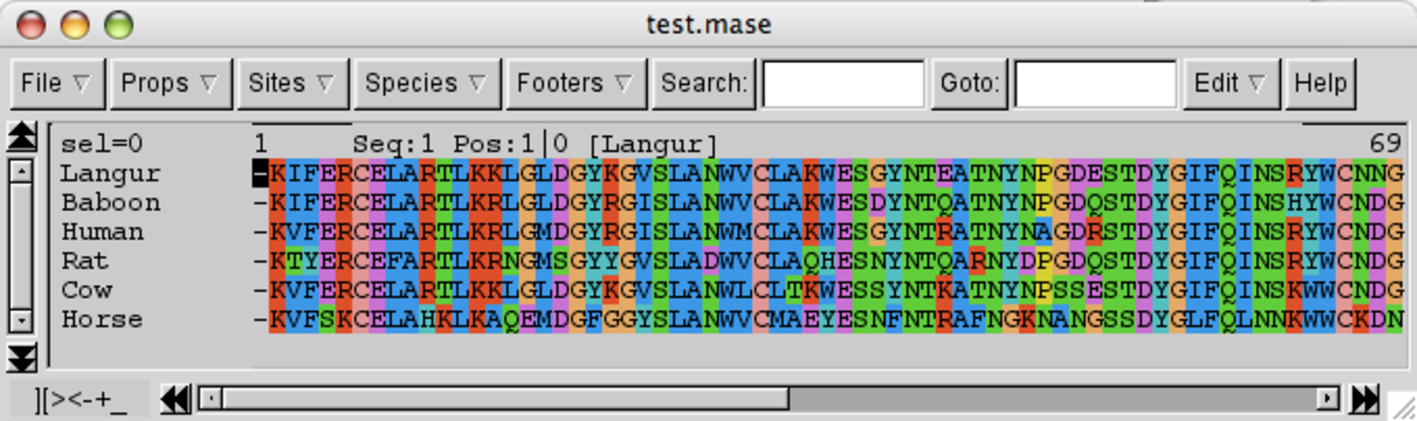
\includegraphics[width=\textwidth]{../figs/SeavView}
\caption{The file \texttt{test.mase} under SeaView. This is a graphical multiple 
sequence alignment editor developped by Manolo Gouy \cite{SeaView}. SeaView 
is able to read and write various alignment formats (NEXUS, MSF, CLUSTAL, 
FASTA, PHYLIP, MASE). It allows to manually edit the alignment, and also to 
run DOT-PLOT or CLUSTALW programs to locally improve the alignment.}
\label{SeaView}
\end{figure}

\subsubsection{clustal}

The CLUSTAL format (*.aln) is the format of the ClustalW multialignment tool 
output \cite{clustalw, clustal2005}. It can be described as follows. The word CLUSTAL is on the first line of 
the file. The alignment is displayed in blocks of a fixed length, each line in the 
block corresponding to one sequence. Each line of each block starts with the 
sequence name (maximum of 10 characters), followed by at least one space 
character. The sequence is then displayed in upper or lower cases, '-' denotes gaps. 
The residue number may be displayed at the end of the first line of each block.

\begin{Schunk}
\begin{Sinput}
 clustalf <- system.file("sequences/test.aln", package = "seqinr")
 cat(readLines(clustalf), sep = "\n")
\end{Sinput}
\begin{Soutput}
CLUSTAL W (1.82) multiple sequence alignment


FOSB_MOUSE      MFQAFPGDYDSGSRCSSSPSAESQYLSSVDSFGSPPTAAASQECAGLGEMPGSFVPTVTA 60
FOSB_HUMAN      MFQAFPGDYDSGSRCSSSPSAESQYLSSVDSFGSPPTAAASQECAGLGEMPGSFVPTVTA 60
                ************************************************************

FOSB_MOUSE      ITTSQDLQWLVQPTLISSMAQSQGQPLASQPPAVDPYDMPGTSYSTPGLSAYSTGGASGS 120
FOSB_HUMAN      ITTSQDLQWLVQPTLISSMAQSQGQPLASQPPVVDPYDMPGTSYSTPGMSGYSSGGASGS 120
                ********************************.***************:*.**:******

FOSB_MOUSE      GGPSTSTTTSGPVSARPARARPRRPREETLTPEEEEKRRVRRERNKLAAAKCRNRRRELT 180
FOSB_HUMAN      GGPSTSGTTSGPGPARPARARPRRPREETLTPEEEEKRRVRRERNKLAAAKCRNRRRELT 180
                ****** ***** .**********************************************

FOSB_MOUSE      DRLQAETDQLEEEKAELESEIAELQKEKERLEFVLVAHKPGCKIPYEEGPGPGPLAEVRD 240
FOSB_HUMAN      DRLQAETDQLEEEKAELESEIAELQKEKERLEFVLVAHKPGCKIPYEEGPGPGPLAEVRD 240
                ************************************************************

FOSB_MOUSE      LPGSTSAKEDGFGWLLPPPPPPPLPFQSSRDAPPNLTASLFTHSEVQVLGDPFPVVSPSY 300
FOSB_HUMAN      LPGSAPAKEDGFSWLLPPPPPPPLPFQTSQDAPPNLTASLFTHSEVQVLGDPFPVVNPSY 300
                ****:.******.**************:*:**************************.***

FOSB_MOUSE      TSSFVLTCPEVSAFAGAQRTSGSEQPSDPLNSPSLLAL 338
FOSB_HUMAN      TSSFVLTCPEVSAFAGAQRTSGSDQPSDPLNSPSLLAL 338
                ***********************:**************
\end{Soutput}
\end{Schunk}

\subsubsection{phylip}

PHYLIP is a tree construction program \cite{PHYLIP}. The format is as follows: the number of 
sequences and their length (in characters) is on the first line of the file. The 
alignment is displayed in an interleaved or sequential format. The sequence 
names are limited to 10 characters and may contain blanks.

\begin{Schunk}
\begin{Sinput}
 phylipf <- system.file("sequences/test.phylip", package = "seqinr")
 cat(readLines(phylipf), sep = "\n")
\end{Sinput}
\begin{Soutput}
  5    42
Turkey    AAGCTNGGGC ATTTCAGGGT
Salmo gairAAGCCTTGGC AGTGCAGGGT
H. SapiensACCGGTTGGC CGTTCAGGGT
Chimp     AAACCCTTGC CGTTACGCTT
Gorilla   AAACCCTTGC CGGTACGCTT

GAGCCCGGGC AATACAGGGT AT
GAGCCGTGGC CGGGCACGGT AT
ACAGGTTGGC CGTTCAGGGT AA
AAACCGAGGC CGGGACACTC AT
AAACCATTGC CGGTACGCTT AA
\end{Soutput}
\end{Schunk}

\subsubsection{msf}

MSF is the multiple sequence alignment format of the GCG sequence analysis 
package (\url{http://www.accelrys.com/products/gcg/index.html}). 
It begins with the line (all uppercase) 
!!NA\_MULTIPLE\_ALIGNMENT 1.0 for nucleic acid sequences or 
!!AA\_MULTIPLE\_ALIGNMENT 1.0 for amino acid sequences. Do not edit 
or delete the file type if its present (optional). A description line which 
contains informative text describing what is in the file. You can add 
this information to the top of the MSF file using a text editor (optional). 
A dividing line which contains the number of bases or residues in the 
sequence, when the file was created, and importantly, two dots (..) 
which act as a divider between the descriptive information and the 
following sequence information (required). msf files contain some other 
information: the Name/Weight, a Separating Line which must 
include two slashes (//) to divide the name/weight information 
from the sequence alignment (required) and the multiple 
sequence alignment.

\begin{Schunk}
\begin{Sinput}
 msff <- system.file("sequences/test.msf", package = "seqinr")
 cat(readLines(msff), sep = "\n")
\end{Sinput}
\begin{Soutput}
PileUp of: @Pi3k.Fil

Symbol comparison table: GenRunData:Pileuppep.Cmp  CompCheck: 1254

                   GapWeight: 3.000
             GapLengthWeight: 0.100 

 Pi3k.Msf  MSF: 377  Type: P  July 12, 1996 10:40  Check: 167 ..

 Name: Tor1_Yeast       Len:   377  Check: 7773  Weight:  1.00
 Name: Tor2_Yeast       Len:   377  Check: 8562  Weight:  1.00
 Name: Frap_Human       Len:   377  Check: 9129  Weight:  1.00
 Name: Esr1_Yeast       Len:   377  Check: 8114  Weight:  1.00
 Name: Tel1_Yeast       Len:   377  Check: 1564  Weight:  1.00
 Name: Pi4k_Human       Len:   377  Check: 8252  Weight:  1.00
 Name: Stt4_Yeast       Len:   377  Check: 9117  Weight:  1.00
 Name: Pik1_Yeast       Len:   377  Check: 3455  Weight:  1.00
 Name: P3k1_Soybn       Len:   377  Check: 4973  Weight:  1.00
 Name: P3k2_Soybn       Len:   377  Check: 4632  Weight:  1.00
 Name: Pi3k_Arath       Len:   377  Check: 3585  Weight:  1.00
 Name: Vp34_Yeast       Len:   377  Check: 5928  Weight:  1.00
 Name: P11a_Human       Len:   377  Check: 6597  Weight:  1.00
 Name: P11b_Human       Len:   377  Check: 8486  Weight:  1.00

//

            1                                                   50
Tor1_Yeast  .......GHE DIRQDSLVMQ LFGLVNTLLK NDSECFKRHL DIQQYPAIPL 
Tor2_Yeast  .......GHE DIRQDSLVMQ LFGLVNTLLQ NDAECFRRHL DIQQYPAIPL 
Frap_Human  .......GHE DLRQDERVMQ LFGLVNTLLA NDPTSLRKNL SIQRYAVIPL 
Esr1_Yeast  .......KKE DVRQDNQYMQ FATTMDFLLS KDIASRKRSL GINIYSVLSL 
Tel1_Yeast  .KALMKGSND DLRQDAIMEQ VFQQVNKVLQ NDKVLRNLDL GIRTYKVVPL 
Pi4k_Human  ..AAIFKVGD DCRQDMLALQ IIDLFKNIFQ LV....GLDL FVFPYRVVAT 
Stt4_Yeast  ..AAIFKVGD DCRQDVLALQ LISLFRTIWS SI....GLDV YVFPYRVTAT 
Pik1_Yeast  ...VIAKTGD DLRQEAFAYQ MIQAMANIWV KE....KVDV WVKRMKILIT 
P3k1_Soybn  TCKIIFKKGD DLRQDQLVVQ MVSLMDRLLK LE....NLDL HLTPYKVLAT 
P3k2_Soybn  ....IFKKGD DIRQDQLVVQ MVSLMDRLLK LE....NLDL HLTPYKVLAT 
Pi3k_Arath  ..KLIFKKGD DLRQDQLVVQ MVWLMDRLLK LE....NLDL CLTPYKVLAT 
Vp34_Yeast  .YHLMFKVGD DLRQDQLVVQ IISLMNELLK NE....NVDL KLTPYKILAT 
P11a_Human  ...IIFKNGD DLRQDMLTLQ IIRIMENIWQ NQ....GLDL RMLPYGCLSI 
P11b_Human  ...VIFKNGD DLRQDMLTLQ MLRLMDLLWK EA....GLDL RMLPYGCLAT 

            51                                                 100
Tor1_Yeast  SPKSGLLGWV PNSDTFHVLI REHRDAKKIP LNIEHWVMLQ MAPDYENLTL 
Tor2_Yeast  SPKSGLLGWV PNSDTFHVLI REHREAKKIP LNIEHWVMLQ MAPDYDNLTL 
Frap_Human  STNSGLIGWV PHCDTLHALI RDYREKKKIL LNIEHRIMLR MAPDYDHLTL 
Esr1_Yeast  REDCGILEMV PNVVTLRSIL STKYESLKIK Y.....SLKS LHDRWQHTAV 
Tel1_Yeast  GPKAGIIEFV ANSTSLHQIL SKLHTNDKIT FDQARKGMKA VQTKSN.... 
Pi4k_Human  APGCGVIECI PDCTS..... .......... RDQLGRQTDF GMYDYFTRQY 
Stt4_Yeast  APGCGVIDVL PNSVS..... .......... RDMLGREAVN GLYEYFTSKF 
Pik1_Yeast  SANTGLVETI TNAMSVHSIK KALTKKMIED AELDDKGGIA SLNDHFLRAF 
P3k1_Soybn  GQDEGMLEFI P.SRSLAQI. .......... ..LSENRSII SYLQ...... 
P3k2_Soybn  GQDEGMLEFI P.SRSLAQI. .......... ..LSENRSII SYLQ...... 
Pi3k_Arath  GHDEGMLEFI P.SRSLAQI. .......... ..LSEHRSIT SYLQ...... 
Vp34_Yeast  GPQEGAIEFI P.NDTLASI. .......... ..LSKYHGIL GYLK...... 
P11a_Human  GDCVGLIEVV RNSHTIMQI. .......... ..Q.CKGGLK GALQFNSHTL 
P11b_Human  GDRSGLIEVV STSETIADI. .......... ..QLNSSNVA AAAAFNKDAL 
\end{Soutput}
\end{Schunk}

\subsubsection{FASTA}

Sequence in fasta format begins with a single-line description (distinguished 
by a greater-than (>) symbol), followed by sequence data on the next line.

\begin{Schunk}
\begin{Sinput}
 fastaf <- system.file("sequences/Anouk.fasta", package = "seqinr")
 cat(readLines(fastaf), sep = "\n")
\end{Sinput}
\begin{Soutput}
>LmjF01.0030
ATGATGTCGGCCGAGCCGCCGTCGTCGCAGCCGTACATCAGCGACGTGCTGCGGCGGTAC
CAGCTGGAGCGCTTTCAGTGTGCCTTTGCATCGAGCATGACCATCAAGGACCTCCTCGCC
CTGCAGCCAGAGGACTTCAACCGCTACGGCGTCGTAGAGGCGATGGACATTTTGCGGCTG
CGTGACGCCATCGAGTACATCAAGGCTAATCCGCTCCCCGCCTCGCGCTCTGGCAGTGAC
GTGCTCGACAACGACGGCGACGGCGACGGCGACGACAGTACGCCGGAGGGGAAGGAGGGG
TGCTCGACGGAGCGCCGGCGGCAGTACACAGCACGCGGAACCACAGTCCTTTGCCGGTCG
ACCGACACCGCCGAGGAGGTGAAGCGCAAGAGCCGCATCCTCGTCGCCATTCGCAAGCGT
CCGCTCAGCGCCGGGGAGCAGACGAACGGCTTCACGGACATCATGGACGCCGACAACAGC
GGCGAGATTGTGCTGAAGGAGCCAAAGGTGAAGGTCGACCTCCGCAAGTACACCCACGTG
CACCGCTTCTTCTTCGACGAGGTTTTCGACGAGGCCTGCGACAACGTCGACGTGTACAAC
CGCGCTGCCCGCGCGCTGATCGACACCGTCTTCGACGGCGGCTGCGCGACATGCTTCGCC
TATGGACAGACAGGGAGCGGCAAGACACACACGATGCTGGGCAAGGGCCCCGAGCCGGGC
CTCTACGCACTCGCCGCCAAAGACATGTTTGACCGCCTCACGAGCGACACGCGCATCGTC
GTTTCCTTTTACGAGATCTACAGCGGGAAGCTCTTTGACTTGCTGAACGGCCGGCGACCC
CTGCGAGCCCTCGAGGACGACAAGGGCCGGGTGAACATCCGCGGCCTCACCGAACACTGC
TCTACCAGCGTGGAGGACCTCATGACGATCATCGACCAGGGCAGCGGTGTTCGCAGCTGC
GGCTCCACCGGCGCCAATGACACAAGCTCCCGCTCCCACGCCATTCTCGAGATCAAGCTC
AAGGCGAAACGGACGTCGAAGCAGAGCGGCAAGTTCACGTTCATCGACCTCGCTGGAAGC
GAGCGCGGCGCTGACACGGTGGACTGCGCGCGACAGACACGCCTCGAAGGGGCGGAGATC
AACAAGAGCCTACTCGCGCTGAAGGAGTGCATTCGTTTTTTAGATCAGAACAGGAAGCAC
GTCCCGTTCCGCGGCTCGAAGCTGACTGAGGTGCTCCGCGACTCGTTTATCGGCAACTGC
CGCACGGTGATGATCGGCGCCGTCTCTCCGTCGAACAACAATGCCGAGCACACGCTGAAC
ACGCTGCGCTACGCCGATCGTGTCAAGGAGCTGAAGCGCAACGCCACGGAGCGGCGCACT
GTGTGCATGCCCGACGACCAGGAAGAGGCCTTCTTTGACACGACCGAGAGCAGGCCACCG
TCGCGGAGGACGACAACTCGCCTTTCTACGGCCGCCCCGCTTTTCTCCGGCTCTTCGACG
GCTGCGCCAGCACTTAGAAGCACGCTACTCAGCAGCCGCTCCGTCAACACACTCTCGCCG
TCGTCGCAGGCCAAGTCGACTCTCGTCACCCCGAAGCCGCCGTCGCGCGATCGGACTCCG
GACATGGTGTGCACTAAGCGGCCCCGCGACTCAGACAGAAGCGGCGAGGACGAAGTGGTA
GCGCGGCCGAGTGGGCGCCCAAGCTTCAAGCGCTTCGAGAGCGGCGCCGAGCTTGTCGCG
GCCCAGCGCAGTCGCGTCATTGACCAATACAACGCCTACCTCGAGACGGACATGAACTGT
ATCAAGGAGGAGTACCAGGTGAAGTACGACGCAGAGCAGATGAACGCCAACACGCGCAGC
TTTGTGGAGCGCGCACGTCTGCTGGTGAGCGAGAAACGGCGCGCGATGGAGTCCTTCCTA
ACGCAGCTGGAGGAGCTCGACAAGATCGCGCAGCAGGTCGCCGACATCACCGCCTTTCAG
CAGCACCTGCCGCCAACG
>LinJ01.0030
ATGATGTCGGCCGAGCCGCCGTCGTCGCAGCCGTACATCAGCGACGTGCTGCGGCGGTAC
CAGCTGGAGCGCTTTCAGAGTTCCTTTGCATCGAGCATGACCATCAAGGACCTCCTCGCC
CTGCAGCCGGAGGACTTCAACCGCTACGGCGTCGTAGAGGCAATGGACATTTTGCGGCTG
CGCGACGCCATCGAGTACATCAAGGCCAACCCGCTCCCCGCCTCGCGCTCCGGCAGTGAC
GTGCTCGACAACGACGGCGACGGCGACGGCGACGACAGTACGCCGGAGGGGAAGGAGGGG
TGCTCGACGGAGCGCCGACGGCAGTACACAGCACGCGGAACCACCGTCCTTTGCGGGTCG
ACCGACACCGCCGAGGAGGTGAAGCGCAAGAGCCGCATCATCGTCGCCATTCGCAAGCGT
CCGCTCAGCGCCGGGGAGCAGACGAACGGCTTCACGGACATCATGGACGCCGACAACAAC
GGCGAGATTGTGCTGAAGGAGCCAAAGGTGAAGGTCGACCTCCGCAAGTACACCCACGTG
CACCGCTTCTTCTTCGACGAGGTTTTCGACGAGGCGTGCGACAACGTCGACGTGTACAAC
CGCGCTGCCCGCGCGCTGATCGACACCGTCTTCGACGGCGGCTGCGCGACATGCTTCGCC
TATGGGCAGACAGGGAGCGGCAAGACACACACGATGCTCGGCAAGGGCCCCGAGCCGGGC
CTGTACGCACTCGCCGCCAAAGACATGTTTGACCGCCTCACGAGCGACACGCGCATCGTT
GTTTCCTTTTACGAGATCTACAGCGGGAAGCTCTTTGACTTGCTGAACGGCCGGCGACCA
CTGCGAGCCCTCGAGGACGACAAGGGGAGGGTGAACATCCGCGGCCTCACCGAACACTGC
TCTACCAGCGTGGAGGACCTCATGACGATCATCGACCAGGGCAGCGGCGTTCGCAGCTGC
GGCTCCACCGGCGCCAACGACACGAGCTCCCGCTCCCACGCCATTCTCGAGATCAAGCTC
AAGGCGAAACGGACGTCGAAGCAGAGCGGCAAGTTCACATTCATCGACCTCGCTGGAAGC
GAGCGCGGCGCCGACACGGTGGATTGCGCGCGACAGACACGCCTCGAAGGGGCGGAGATT
AACAAGAGCCTACTCGCTCTGAAGGAGTGCATTCGTTTTTTAGATCAGAACAGGAAGCAC
GTCCCGTTCCGCGGCTCGAAGCTGACTGAGGTGCTCCGCGACTCGTTTATCGGCAACTGC
CGCACGGTGATGATCGGCGCCGTCTCTCCGTCCAACAACAATGCCGAGCACACGCTGAAC
ACGTTGCGCTACGCCGATCGCGTCAAGGAGCTGAAGCGCAACGCCACGGAGCGGCGCACC
GTGTGCGTGCCCAACGACCAGGAAGAGGCCTTCTTTGACACGACCGAGAGCAGGCCACCG
TCGCGGAGGACGACAACTCGGCTTTCTGCGGCCGCCCCGCTTTTCTCCGGCACTTCGACG
GCTGCCCCAGCATGTAAAAGCACGTTGCTCAGCAGCCGCTCCGTCAACACACTCTCGCCG
TCGTCGCAGGGCAAGTCGACTCTCGTCACCCCGAAGCCACTGTCGCGCGATCGGACTCCG
GACATGGTGTGCGCTAAGCGGCCCCGCGACTCAGACCGAAGCGGCGAAGACGAAGTGGTG
GCGCGGCCGAGTGGGCGCCCAAGCTTCAAGCGCTTCGAGGGCGGCGCCGAGCTCGTGGCG
GCCCAGCGCAGTCGTGTCATTGACCAATACAACGCCTACCTCGAGACGGACATGAACTGT
ATCAAGGAGGAGTACCAGGTGAAGTACGACGCAGAGCAGATGAACGCCAACACGCGCACC
TTTGTCGAGCGCGCACGCCTGCTGGTGAGCGAGAAGCGGCGCGCGATGGAGTCCTTCCTA
ACGCAGCTGGACGAGCTCGATAAGATCGCGCAGCAGGTCGCCAGCATCACCGCCTTTCAG
CAGCACCTGCCGCCAACG
\end{Soutput}
\end{Schunk}

\subsection{The function \texttt{read.alignment()}}

Aligned sequence data are very important in evolutionary studies,
in this representation all vertically aligned positions are supposed
to be homologous, that is sharing a common ancestor. This is a
mandatory starting point for comparative studies. 
There is a function in \seqinr{} called \texttt{read.alignment()} to 
read aligned sequences data from various formats  (\texttt{mase}, 
\texttt{clustal}, \texttt{phylip}, \texttt{fasta} or \texttt{msf})
produced by common external programs for multiple sequence alignment.

\begin{Schunk}
\begin{Sinput}
 example(read.alignment)
\end{Sinput}
\begin{Soutput}
rd.lgn mase <- read.alignment(file = system.file("sequences/test.mase", package = "seqinr"), format = "mase")

rd.lgn clustal <- read.alignment(file = system.file("sequences/test.aln", package = "seqinr"), format="clustal")

rd.lgn phylip <- read.alignment(file = system.file("sequences/test.phylip", package = "seqinr"), format = "phylip")

rd.lgn msf <- read.alignment(file = system.file("sequences/test.msf", package = "seqinr"), format = "msf")

rd.lgn fasta <- read.alignment(file = system.file("sequences/Anouk.fasta", package = "seqinr"), format = "fasta")
\end{Soutput}
\end{Schunk}

%The data returned by \texttt{read.alignment()} are of class
%alignment. Whereas sequences are stored as vector of character for the
%class \texttt{"SeqFastadna"}, \texttt{"SeqFastaAA"} and  \texttt{"SeqAcnucWeb"},
%they are stored as vector of strings for the class \texttt{"alignment"}.

\subsection{A simple example with the louse-gopher data}

Let's give an example. The gene coding for the mitochondrial cytochrome oxidase I 
is essential and therefore often used in phylogenetic studies because of its
ubiquitous nature. The following two sample tests
of aligned sequences of this gene (extracted from ParaFit \cite{parafit}), 
are distributed along with the \seqinr{} package:

\begin{Schunk}
\begin{Sinput}
 louse <- read.alignment(system.file("sequences/louse.fasta", 
     package = "seqinr"), format = "fasta")
 louse$nam
\end{Sinput}
\begin{Soutput}
[1] "gi|548117|gb|L32667.1|GYDCYTOXIB" "gi|548119|gb|L32668.1|GYDCYTOXIC"
[3] "gi|548121|gb|L32669.1|GYDCYTOXID" "gi|548125|gb|L32671.1|GYDCYTOXIF"
[5] "gi|548127|gb|L32672.1|GYDCYTOXIG" "gi|548131|gb|L32675.1|GYDCYTOXII"
[7] "gi|548133|gb|L32676.1|GYDCYTOXIJ" "gi|548137|gb|L32678.1|GYDCYTOXIL"
\end{Soutput}
\begin{Sinput}
 gopher <- read.alignment(system.file("sequences/gopher.fasta", 
     package = "seqinr"), format = "fasta")
 gopher$nam
\end{Sinput}
\begin{Soutput}
[1] "gi|548223|gb|L32683.1|PPGCYTOXIA" "gi|548197|gb|L32686.1|OGOCYTOXIA"
[3] "gi|548199|gb|L32687.1|OGOCYTOXIB" "gi|548201|gb|L32691.1|OGOCYTOXIC"
[5] "gi|548203|gb|L32692.1|OGOCYTOXID" "gi|548229|gb|L32693.1|PPGCYTOXID"
[7] "gi|548231|gb|L32694.1|PPGCYTOXIE" "gi|548205|gb|L32696.1|OGOCYTOXIE"
\end{Soutput}
\end{Schunk}

\begin{figure}[htbp]
   \begin{center}
   \begin{tabular}{cc}
      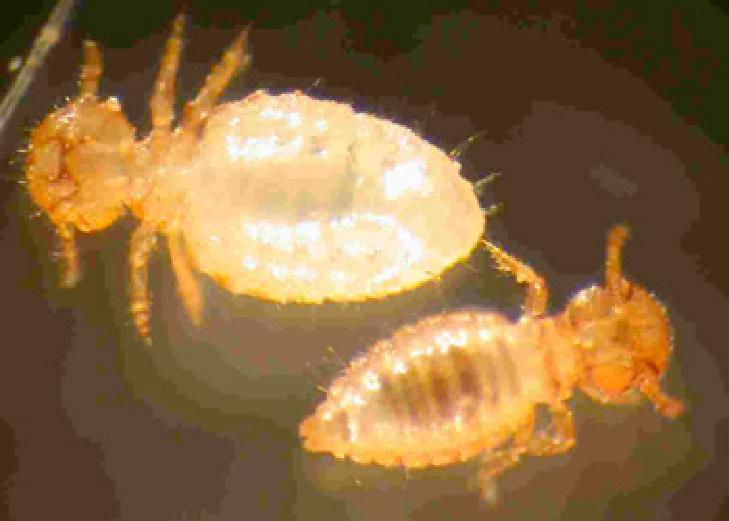
\includegraphics[width=0.5\textwidth]{../figs/louse}&
      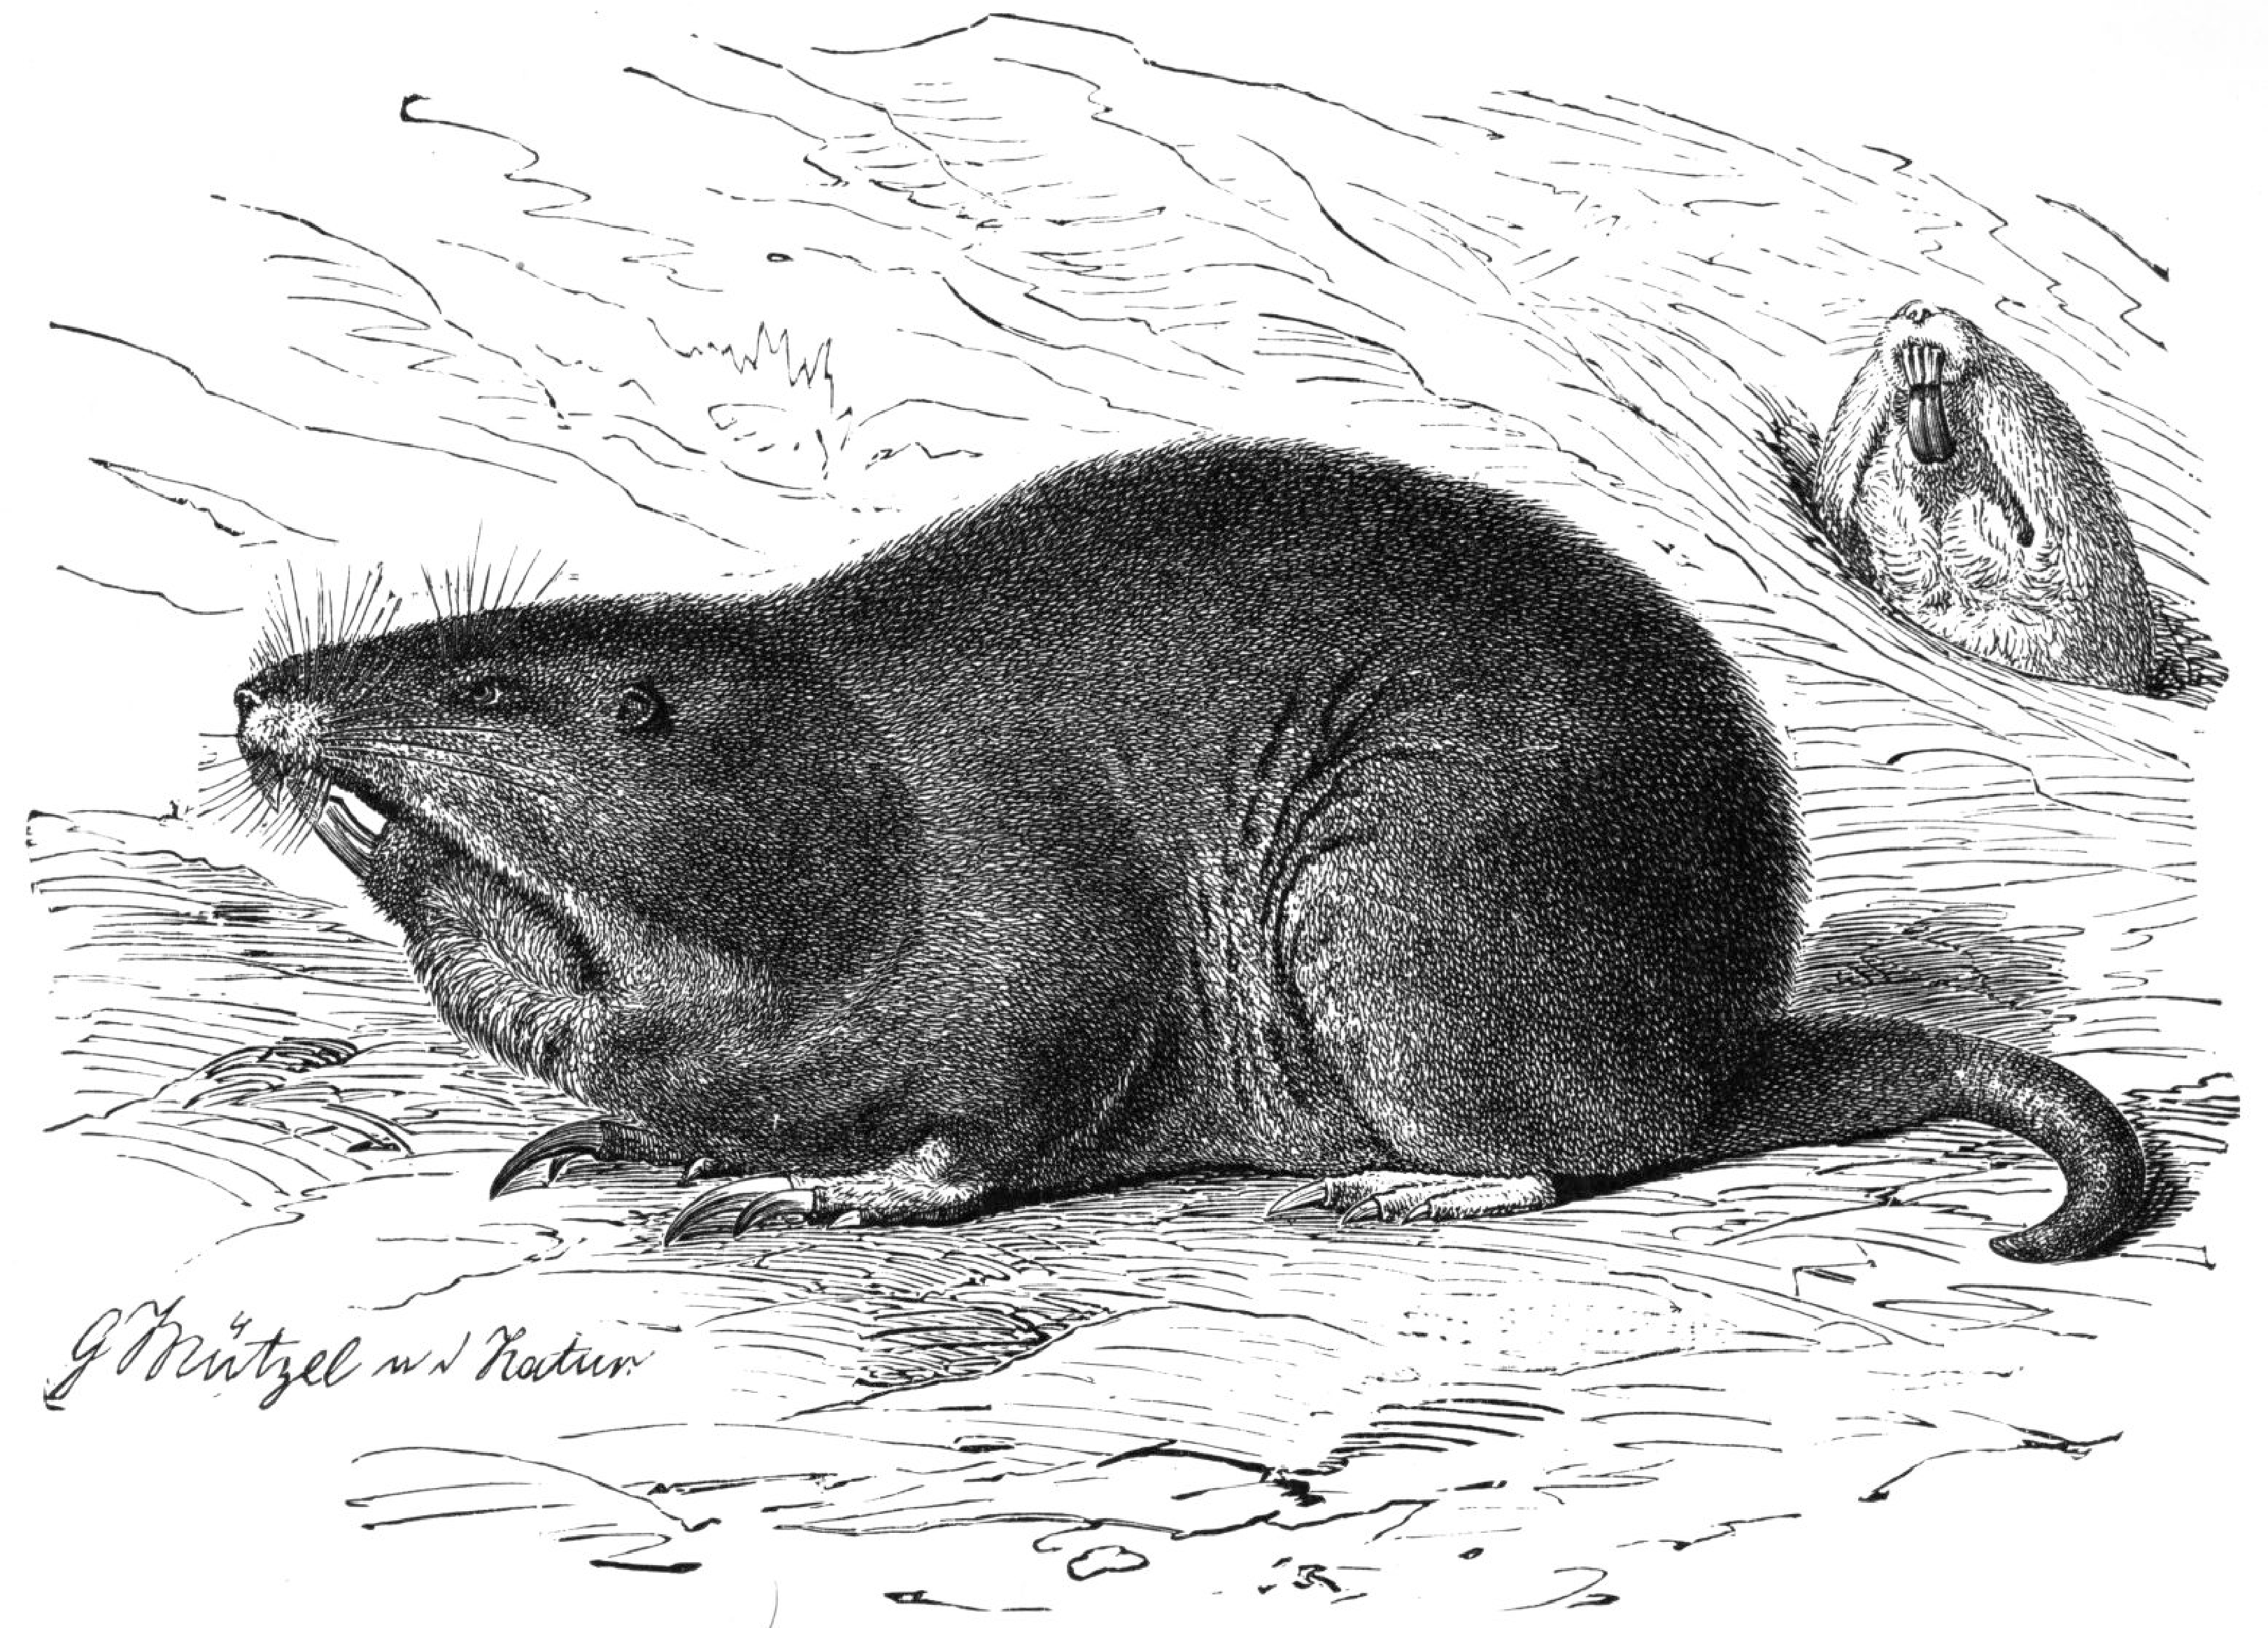
\includegraphics[width=0.5\textwidth]{../figs/gopher}\\
   \end{tabular}
   \end{center}
   \caption{Louse (left) and gopher (right). 
   Images are from the wikipedia (\protect\url{http://www.wikipedia.org/}).
   The picture of the chewing louse \textit{Damalinia limbata} found on Angora goats
   was taken by Fiorella Carnevali (ENEA, Italy). The gopher drawing is from
   Gustav M{\"u}tzel, Brehms Tierleben, Small Edition 1927.}
   \label{lousegopher}
\end{figure}

The aligned sequences are now imported in your \Rlogo{}~environment.
The $8$ genes of the first sample are from various species of louse (insects parasitics
on warm-blooded animals) and the $8$ genes of the second sample are from their corresponding
gopher hosts (a subset of rodents), see figure \ref{lousegopher} :

\begin{Schunk}
\begin{Sinput}
 l.names <- readLines(system.file("sequences/louse.names", 
     package = "seqinr"))
 l.names
\end{Sinput}
\begin{Soutput}
[1] "G.chapini "  "G.cherriei " "G.costaric " "G.ewingi  "  "G.geomydis "
[6] "G.oklahome " "G.panamens " "G.setzeri  "
\end{Soutput}
\begin{Sinput}
 g.names <- readLines(system.file("sequences/gopher.names", 
     package = "seqinr"))
 g.names
\end{Sinput}
\begin{Soutput}
[1] "G.brevicep " "O.cavator "  "O.cherriei " "O.underwoo " "O.hispidus "
[6] "G.burs1 "    "G.burs2 "    "O.heterodu" 
\end{Soutput}
\end{Schunk}

\Seqinr{} has very few methods devoted to phylogenetic analyses but many are
available in the \texttt{ape} package \cite{ape2004}. This allows for a very fine tuning
of the graphical outputs of the analyses thanks to the power of the \Rlogo{}
facilities. For instance, a natural question
here would be to compare the topology of the tree of the hosts and their
parasites to see if we have congruence between host and parasite evolution.
In other words, we want to display two phylogenetic trees face to face. This
would be tedious with a program devoted to the display of a single phylogenetic
tree at time, involving a lot of manual copy/paste operations, hard to reproduce,
and then boring to maintain with data updates.

How does it looks under \Rlogo{}? First, we need to \emph{infer} the 
tree topologies
from data. Let's try as an \emph{illustration} the famous neighbor-joining tree estimation 
of Saitou and Nei \cite{nj} with Jukes and Cantor's correction \cite{JC}
for multiple substitutions.

\begin{Schunk}
\begin{Sinput}
 library(ape)
 louse.JC <- dist.dna(as.DNAbin(louse), model = "JC69")
 gopher.JC <- dist.dna(as.DNAbin(gopher), model = "JC69")
 l <- nj(louse.JC)
 g <- nj(gopher.JC)
\end{Sinput}
\end{Schunk}

Now we have an estimation for \emph{illustrative} purposes of the tree topology for the parasite 
and their hosts. We want to plot the two trees face to face, and for this we must change 
R graphical parameters. The first thing to do is to save the current graphical parameter
settings so as to be able to restore them later:

\begin{Schunk}
\begin{Sinput}
 op <- par(no.readonly = TRUE)
\end{Sinput}
\end{Schunk}

The meaning of the \texttt{no.readonly = TRUE} option here is that graphical
parameters are not all settable, we just want to save those we can change at will. Now,
we can play with graphics :

\setkeys{Gin}{width=\textwidth}
\begin{Schunk}
\begin{Sinput}
 g$tip.label <- paste(1:8, g.names)
 l$tip.label <- paste(1:8, l.names)
 layout(matrix(data = 1:2, nrow = 1, ncol = 2), width = c(1.4, 
     1))
 par(mar = c(2, 1, 2, 1))
 plot(g, adj = 0.8, cex = 1.4, use.edge.length = FALSE, main = "gopher (host)", 
     cex.main = 2)
 plot(l, direction = "l", use.edge.length = FALSE, cex = 1.4, 
     main = "louse (parasite)", cex.main = 2)
\end{Sinput}
\end{Schunk}
\includegraphics{../figs/getseqflat-face2face}
\setkeys{Gin}{width=0.8\textwidth}

We now restore the old graphical settings that were previously saved:

\begin{Schunk}
\begin{Sinput}
 par(op)
\end{Sinput}
\end{Schunk}

OK, this may look a little bit obscure if you are not fluent in programming, but please
try the following experiment. In your current working directory, that is in the
directory given by the \texttt{getwd()} command, create a text file called
\texttt{essai.r} with your favourite text editor, and copy/paste the previous \Rlogo{}
commands, that is :

\tiny
\begin{verbatim}
louse <- read.alignment(system.file("sequences/louse.fasta", package = "seqinr"), format = "fasta")
gopher <- read.alignment(system.file("sequences/gopher.fasta", package = "seqinr"), format = "fasta")
l.names <- readLines(system.file("sequences/louse.names", package = "seqinr"))
g.names <- readLines(system.file("sequences/gopher.names", package = "seqinr"))
library(ape)
louse.JC <- dist.dna(as.DNAbin(louse), model = "JC69")
gopher.JC <- dist.dna(as.DNAbin(gopher), model = "JC69")
l <- nj(louse.JC)
g <- nj(gopher.JC)
g$tip.label <- paste(1:8, g.names)
l$tip.label <- paste(1:8, l.names)
layout(matrix(data = 1:2, nrow = 1, ncol = 2), width=c(1.4, 1))
par(mar=c(2,1,2,1))
plot(g, adj = 0.8, cex = 1.4, use.edge.length=FALSE, 
  main = "gopher (host)", cex.main = 2)
plot(l,direction="l", use.edge.length=FALSE, cex = 1.4,
  main = "louse (parasite)", cex.main = 2)       
\end{verbatim} 
\normalsize

Make sure that your text has been saved and then go back to \Rlogo{}~console to enter
the command :

\scriptsize
\begin{verbatim}
source("essai.r")
\end{verbatim}
\normalsize

This should reproduce the previous face-to-face phylogenetic trees in your \Rlogo{}~graphical device. 
Now, your boss is unhappy with working with the Jukes and Cantor's model \cite{JC}
and wants you to use the Kimura's 2-parameters distance \cite{K80} instead.
Go back to the text editor to change \texttt{model = "JC69"} by \texttt{model = "K80"},
save the file, and in the \Rlogo{}~console \texttt{source("essai.r")} again, you should
obtain the following graph :

\setkeys{Gin}{width=\textwidth}
\includegraphics{../figs/getseqflat-K80}
\setkeys{Gin}{width=0.8\textwidth}

Now, something even worst, there was a error in the
aligned sequence set: the first base in the first sequence in the file
\texttt{louse.fasta} is not a C but a T. To locate the file on your system,
enter the following command:

\begin{Schunk}
\begin{Sinput}
 system.file("sequences/louse.fasta", package = "seqinr")
\end{Sinput}
\begin{Soutput}
[1] "/Users/lobry/seqinr/pkg.Rcheck/seqinr/sequences/louse.fasta"
\end{Soutput}
\end{Schunk}

Open the \texttt{louse.fasta} file
in your text editor, fix the error, go back to the \Rlogo{}~console to
\texttt{source("essai.r")} again. That's all, your graph is now consistent with
the updated dataset.


\section*{Session Informations}

This part was compiled under the following \Rlogo{}~environment:

\begin{itemize}
  \item R version 2.8.0 (2008-10-20), \verb|i386-apple-darwin8.8.2|
  \item Locale: \verb|fr_FR.UTF-8/fr_FR.UTF-8/fr_FR.UTF-8/C/C/C|
  \item Base packages: base, datasets, grDevices, graphics, methods,
    stats, utils
  \item Other packages: MASS~7.2-44, ade4~1.4-9, ape~2.2-2,
    nlme~3.1-89, quadprog~1.4-11, seqinr~2.0-0, tseries~0.10-16,
    xtable~1.5-4, zoo~1.5-4
  \item Loaded via a namespace (and not attached): grid~2.8.0,
    lattice~0.17-15, tools~2.8.0
\end{itemize}
There were two compilation steps:

\begin{itemize}
  \item \Rlogo{} compilation time was: Sun Oct 26 17:53:17 2008
  \item \LaTeX{} compilation time was: \today
\end{itemize}


% END - DO NOT REMOVE THIS LINE

%%%%%%%%%%%%  BIBLIOGRAPHY %%%%%%%%%%%%%%%%%
\clearpage
\addcontentsline{toc}{section}{References}
\bibliographystyle{plain}
\bibliography{../config/book}
\end{document}
